\documentclass[titlepage]{article}
\usepackage{amsmath}
\usepackage{amsfonts}
\usepackage{physics}
\usepackage{graphicx}
\usepackage{hyperref}
\usepackage{cleveref}
\usepackage[backend = bibtex,style=phys, articletitle=false,  biblabel=brackets, sorting=none]{biblatex}
%\usepackage{fullpage}
\usepackage{pythontex}
% Title Page

%\bibliography{chgcnn}
\addbibresource{chgcnn.bib}

\title{Symmetry Group Equivariant Neural Networks for Physical Systems}
\author{Alexander J. Heilman}


\begin{document}
	\maketitle

	
%	\tableofcontents
	
	\section{Literature Review \& Background}
	The fundamental assumption in any mathematical model is that some initial set of properties describing the state of a system fully determines it's future state. And at a high level, it could be argued that both the fields of physics and machine learning are most fundamentally applications of mathematical modeling.
	
	Physics is essentially the pursuit of rigorous mathematical models that accurately describe physical phenomena, mapping some set of physical observables at one point in time to other sets of physical observables at the same or different times. Often these models of physics have some (hopefully intuitive) rationale behind them from which they are derived, but such models must always describe the data collected empirically.
	
	Machine Learning (ML) describes a set of techniques which also assume there exists a map between some input space and some target space (though, perhaps, in an extremely complex manner). However, supervised ML approaches typically start with some sufficiently large, and initially randomly-chosen, model which is then iteratively tuned or 'trained' to better fit the given target data directly. In this way, supervised ML methods are a general tool that allows one to build mathematical models for arbitrary mappings, given sufficient data, from some set of tunable ansatz. Their possible application to physical systems (the same as those modeled by 'pure' physics) should then be obvious.
	
	Indeed, many machine learning techniques have proven to be effective and efficient in many applications to the natural sciences \cite{mlreview1,mlreview1.5,mlreview2,mlreview2.25,mlreview2.5,mlreview2.75,mlreview3}. Of particular interest here are supervised learning techniques applied to the prediction of material properties from atomistic systems (usually DFT-relaxed or idealized), typically crystalline materials \cite{cgcnn, alignn,amdnet,tfn,megnet,m3gnet} or molecules \cite{schnet,molecule0,molecule1,molecule2}.
	
	\subsection{Graph Neural Networks Applied to Atomic Systems}
	One set of machine learning techniques utilizes a general set of mathematical functions referred to as neural networks.
	Neural networks are a class of universal function approximators, composed layer-wise by functions $\mathcal{L}^1\circ\mathcal{L}^2\circ ... \circ \mathcal{L}^n $, where each layer-to-layer transition map $\mathcal{L}^i$ is a trainable function from some feature space associated with layer $L$ to a feature space associated with layer $L+1$ \cite{nn_overview}. While hard proofs of the suitability of machine learning techniques are elusive due to the wide range of both techniques and target spaces, some proofs have been given for suitably wide and deep networks as universal function approximators \cite{universal1, universal2}.
	
	Many modern approaches use a specific type of neural network, referred to as a Graph Neural Network (GNN), which act on data encoded in features associated with some representative graph (i.e. a collection of nodes and connections between them) \cite{gnnintro}. In applications to physical systems, we encode atomic arrangements (such as crystals and molecules) as graphs with associated features and then update their associated features, initially derived from physical properties, through such a graph neural network.
	
	Convolution on graphs (or "message passing" on graphs \cite{MPNN}) is a generalization of typical convolutional networks applied to image-related tasks, such as image classification. In typical convolutional networks, feature maps describing each pixel are updated by the features of their neighborhood of pixels (up to some set size) \cite{cnn_intro}. Through layers of convolution on graph features, features are updated according to their neighboring node's features, with neighbors here defined as nodes sharing edges \cite{cgcnn,congn}.
	
	In typical convolutional networks however, pixels have fixed distances between them, allowing for discretized 'filters' that expect fixed distances between neighborhoods of pixels. In atomic systems though, distances between atoms are continuous and thus require filters sensitive to continuously-distributed features. Such `continuous filters', useful for applications to atomic systems, were first introduced in SchNet \cite{schnet}. The widely-cited Crystal Graph Convolutional Neural Network (CGCNN \cite{cgcnn}) and following works \cite{icgcnn, megnet,alignn} then used continuous filters to great effect on a wide variety of material property prediction tasks.
	
	
	\subsubsection{Crystal Graphs}
	Of course to apply graph neural networks to atomistic systems, such as crystals and molecules, we first require some way to encode these systems in corresponding graphs. We may define a crystal graph $\mathcal{G}=\lbrace \mathcal{V},\mathcal{E}\rbrace$ as a set of vertices $v_i\in\mathcal{V}$, corresponding to each atom $i$, and edges $e_{ij}\in\mathcal{E}$, where edges are determined by some physical criteria. Physical information is then associated with the objects in these graphs by way of feature vectors. These are vectors with components describing the physical characteristics of their corresponding graph component, and are further 'learned' or updated throughout the layers of a graph neural network.
	
	The nodes' feature vectors encode the atomic information of the sites they describe. Two usual techniques include: explicitly engineered feature vectors (as in \cite{cgcnn}); and the learning of encodings for atomic sites based only on their atomic number (as in \cite{megnet}), beginning with some random initialization. Edge features are often derived exclusively from their corresponding interatomic distance, and expressed as a multidimensional feature vector by way of a Radial Basis Functions (RBF). Common radial basis functions include Gaussian and Bessel expansions, with an example Gaussian RBF given in   \cref{crystalgraph}.
	

	A commonly applied criterion for the formation of edges between atoms is a combination of a maximum distance cutoff $r_{max}$ and a maximum number of neighbors for each node $N_{max}$. That is, for each atom, edges are constructed between its node and its $\leq N_{max}$-th closest neighbors in the crystalline structure within a shell of radius $r_{max}$.
	While other criteria may also be utilized, such as face-sharing in Voronoi Tesselations \cite{voronoi_alg}, and scaled maximum distance cutoffs based on nearest neighbor distances, these more advanced criteria are generally more computationally expensive in the data processing stage and often provide negligible differences in performance. Alternatively, most models \cite{cgcnn,alignn,megnet} adopt the more basic criteria of maximum numbers of neighbors within cutoff shells, and adopt some continuous-filter convolutional function that can learn which connections are more important for the task at hand.
	Often, this maximum number of neighbors considered is chosen to be $12$, however recent tests in coNGN \cite{congn} suggest even this may be too restrictive, and show that a maximum set as large as 24 may improve performance.
	
	\begin{figure}\label{crystalgraph}
		
		\begin{center}
			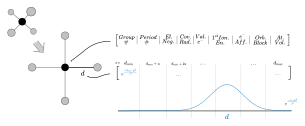
\includegraphics[scale=0.4]{../chgcnn/chgcnn_revised_1/crystal_graph_feat.pdf}
		\end{center}
		
		\caption{Schematic for a simple CGCNN-like graph encoding of some basic atomic structure. Note that the atomic properties are generally expanded by some one-hot encoding or RBF expansion and then concatenated. The edge feature here then is given, as an example, in terms of a Gaussian expansion of $d$, where $d$ is the relevant interatomic spacing.}
	\end{figure}
	
	\subsubsection{Crystal Graph Convolution}
	Crystal graphs are usually constructed solely for use in graph convolutional neural networks. Perhaps the most general framework in which we may define graph convolution is the message passing framework defined by Gilmore \cite{MPNN}.
	A message passing network updates nodes based on 'messages' generated by the features of, and passed through, neighboring nodes (that is, nodes sharing an edge). Gilmore defines the message passing framework in terms of three functions: $M$, the message forming function; $U$, the node update function; and $R$, the readout function. These three functions act on graph representations as follows:
	\begin{gather*}
		m_i^{t+1}=\sum_{n_j\in \mathcal{N}(i)} M_t(n_i^{t},e_{ij},n_j^t )\\
		n_i^{t+1}=U_t(n_i^t,m_i^{t+1})\\
		\hat{y}=R(\lbrace n_v^T\rbrace)
	\end{gather*}
	Where for each pair of connected nodes (or edge), a message is formed from each node's representation $n_i^t,n_j^t$, of layer $t$, and the connecting edge's feature $e_{ij}$. These  node representations of layer $t$ are updated to their $t+1$-th layer representation by update function $U_t$ of layer $t$, which takes as input the set of messages for each node, and the nodes current representation. At the final layer $T$, the readout function $R$ then predicts the target value $\hat{y}$ from the updated node representations.
	
	Message passing networks acting on crystal graphs have several advantages: message passing networks enjoy invariance under permutation of node indices; and, further, if the encoded features are coordinate system invariant, the output of the network is itself coordinate system invariant.
	
	%\subsection{Disadvantages of Crystal Graphs}
	
	However, the graph construction above lacks the inclusion higher-order geometrical information within the crystals. That is, distinct local geometrical environments of atoms (coordination environments/motifs) may be mapped degenerately to the same crystal graph \cite{congn, chgcnn}.
	One could include atomic position in the node features or a vector direction in edge features, however, this generally requires a unique treatment of such coordinate-system dependent information through convolution. As such, often only coordinate system invariant features are included in crystal graph representations, such as distance and atomic properties. 
	Modern approaches that do incorporate coordinate-system dependent features are often \textit{equivariant} by construction, and such equivariant networks are introduced in the following section. 
	
	\subsection{$O(3)$-Equivariant Networks}
%	Graph networks, in their application to atomic systems, are typically coordinate-system invariant by design. That is, the encoding of atomic information and arrangement typically is done in such a way without coordinate-system dependent quantities, instead relying on connectivity and inter-atomic distance to enforce invariance. 
	When a function is claimed to be equivariant, it always is with respect to some group that acts on it's input and output space. For physical space, the most general symmetry group is $O(3)$, the orthogonal group of $\mathbb{R}^3$, containing all rotations and reflections about some central point.
	$O(3)$-Equivariant networks provide a framework in which direction quantities are encoded and, further, respected through convolution; in this way, outputs themselves may be treated as directional quantities. %In general, equivariant functions are functions that preserve the action of a group on it's domain in it's codomain. 
	In essence, equivariant functions commute with their domain and codomain's group representations. More explicitly, for a function $f:X\rightarrow Y$, where $X$ and $Y$ are vector spaces with some set of group representations $\mathcal{D}^{X}(G)$ and $\mathcal{D}^Y(G)$ acting on these spaces respectively, $f$ is equivariant with respect to $G$ if it satisfies:
	$$
	\mathcal{D}^{Y}(g)f(x)=f\big( \mathcal{D}^{X}(g)x\big)
	$$
	Compositions of equivariant functions are themselves equivariant functions \cite{equivariant_cohen}. As such, we may form an equivariant network by composing it layer-wise from a set of equivariant functions. Common choices for such building blocks include: $O(3)$-feature convolutions, $\ell$-wise self-interactions and non-linearities, and pooling across nodes. The most important of these is $O(3)$-equivariant convolution.
	
	Through convolution, convolutional filters and node features interact through tensor products, since
	tensor products of two representation spaces are equivariant under transformation of the two subspaces, i.e.:
	$$
	\mathcal{D}^V\otimes \mathcal{D}^W=\mathcal{D}^{V\otimes W}.
	$$
	By way of Clebsch-Gordan coefficients $c^{\ell_3m_3}_{\ell_1m_1\ell_2m_2}$, these tensor products of $SO(3)$ irreducible representations may be related to a third set of irreducible representations as \cite{e3nn}:
	$$
	(u\otimes v)_{\ell_o}^{m_o} = c_{\ell_1m_1\ell_2m_2}^{\ell_om_o}u_{\ell_1}^{m_1}v_{\ell_2}^{m_2}
	$$
	where $u$ and $v$ are harmonic vectors of order $\ell_1$ and $\ell_2$, respectively.
	Since tensor products of representations are naturally equivariant, $SO(3)$-equivariant convolution is often defined as the scaled tensor product of the two representation spaces (i.e. that of the input feature space, and the filter space). Specifically, layer to layer convolutional maps $\mathcal{L}$ may be defined component-wise as \cite{tensorfieldnetworks}:
	$$
	\mathcal{L}^{\ell_o}_{acm_o}\big(\vec{r}_a,V_{acm_i}^{\ell_i}\big) = \sum_{m_f,m_i}c_{\ell_im_i\ell_fm_f}^{\ell_o m_o}\sum_{b}F^{\ell_f\ell_i}_{cm_f}(r_{ab})V_{bcm_i}^{\ell_i}
	$$
	where the filter function $F^{\ell_f\ell_i}_{cm_f}(r_{ab})$ depends only on the distance between point $a$ and $b$ (as opposed to directional dependence, to maintain equivariance). Instances of such functions then generally have independent, trainable parameters for different rotational orders $\ell_f, \ell_i$, azimuthal orders $m$, and channels $c$. It should be noted that this requires the node and edge features of the graphs to also have these additional indexes in such equivariant networks, as well as the outputs of these networks.
	%To maintain equivariance, for an input feature set of the type described above,  through convolution with some filter $F$,  the filter also must be associated with a set of spherical harmonics, and thus also has an additional two indices $\ell_f$ and $m_f$. 
	
	 
	\section{Current/Previous Work}
	
	My previous work pertains to both invariant  and equivariant graph neural networks in their application to materials science. Particularly, these works focus on improving the expressiveness of invariant graph neural networks by generalizing descriptors to hypergraphs; and utilizing $O(3)$-equivariant networks to predict tensorial material properties. Below, the techniques of both of these previous works are briefly introduced to help further motivate the proposed problem, the statement of which follows this section.
	
	
	\subsection{Crystal Hypergraph Networks}
	The primary problem with the representations of material systems in invariant graph neural networks is that they often lack 'geometrical resolution' beyond interatomic distance. For example, in the proto-typical techniques of CGCNN, distinct coordination environments of the same interatomic-distance and coordination number will be mapped onto equivalent graphs, as displayed in   \cref{fig:graph_cntex}. 
	
	Several approaches have been taken to increase the geometric resolution of invariant graph neural networks: namely, the inclusion of bond-angles as additional triplet features, dihedral angles as quartic features, etc.; and, alternatively, the explicit inclusion of higher-order (than strictly pair-wise) tailored neighborhood features describing common motifs in crystal systems, or more generally, common coordination environments.
	
	
	\begin{figure*}
		\centering
		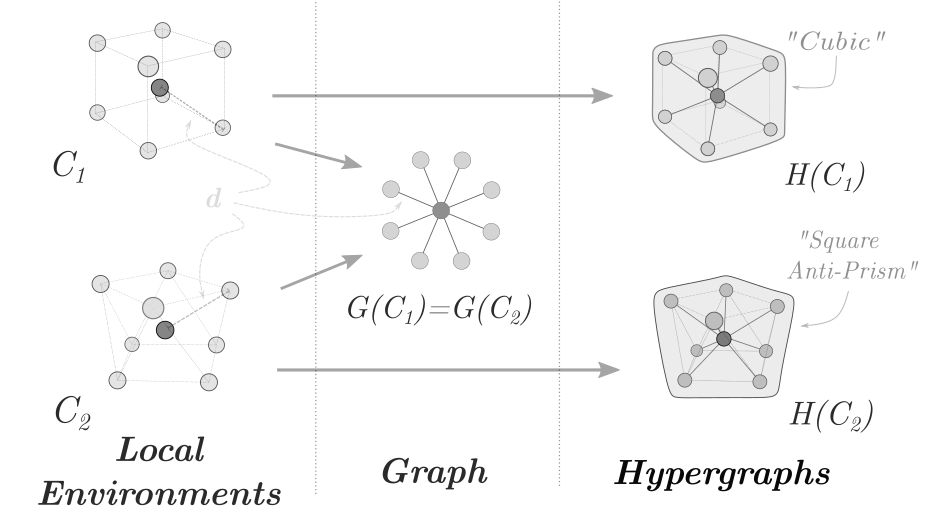
\includegraphics[scale=0.5]{../chgcnn/chgcnn_revised_3/graph2hgraph_tall_revise2.pdf}
		\caption{An example of two distinct geometries that are mapped to the same distance-based crystal graph. With inclusion of a first-shell feature vector encoding local geometry however, these structures are mapped to two distinct crystal hypergraphs. Note these are two possible coordination environments in oxides, determined statistically in \cite{motifstats}.}
		\label{fig:graph_cntex}
	\end{figure*}
	
	
	My approach to increasing geometric resolution, while maintaining invariance, was to extend the graphical descriptions of material systems to hypergraph descriptions, in which edges (now hyperedges) are then allowed to contain more than two atoms. This allows for all invariant features to be naturally associated with arbitrary order structures in materials, simultaneously on equal footing. For example, pairs, triplets, and coordination environments may all be described in the same crystal hypergraph as hyperedges of differing orders.
	
	
	
	
	\subsubsection{Crystal Hypergraphs}
	Hypergraphs are a very general framework describing relations between an abstract set $\mathcal{V}$ of nodes or vertices, defined by by a set of hyperedges $\mathcal{H}$ containing arbitrary subsets of $\mathcal{V}$. Consequently, the set of all hypergraphs on a set of nodes is more general than, and contains all possible, topological sets and simplicial complexes on $\mathcal{V}$ \cite{Mulas2022}. The method proposed here reduces the intrinsic limitations of invariant crystal graph features by allowing the explicit incorporation of higher-order geometrical information in the form of hyperedges, which can be used to directly represent these higher-order structures.
	
	
	
	A crystal hypergraph $\mathcal{H}=\lbrace\mathcal{V}, \mathit{H} \rbrace$ is a collection of nodes $v_i\in \mathcal{V}$ and hyperedges $h_j\in \mathit{H}$ (containing an arbitrary number of nodes, see Supplementary Note S5), where the hyperedges are most generally heterogeneous. That is, we generally wish to describe different types of hyperedges (e.g. bonds, triplets, and motifs) in the same crystal hypergraph. These objects then have associated feature vectors encoding relevant physical information, which we also refer to as $v_i$ and $h_j$, since the indices specify all the relevant information for their association to particular nodes and hyperedges, respectively.
	
	For the purpose of modeling material systems, we need to identify what different order structures are most important in their representation. Of course, atomic and bond level information is particularly important. However, higher-order structures may also be of interest, such as triplets of atoms and local environments of atoms, which we refer to as motifs in crystals.
	
	
	\begin{figure*}[!ht]
		\centering
		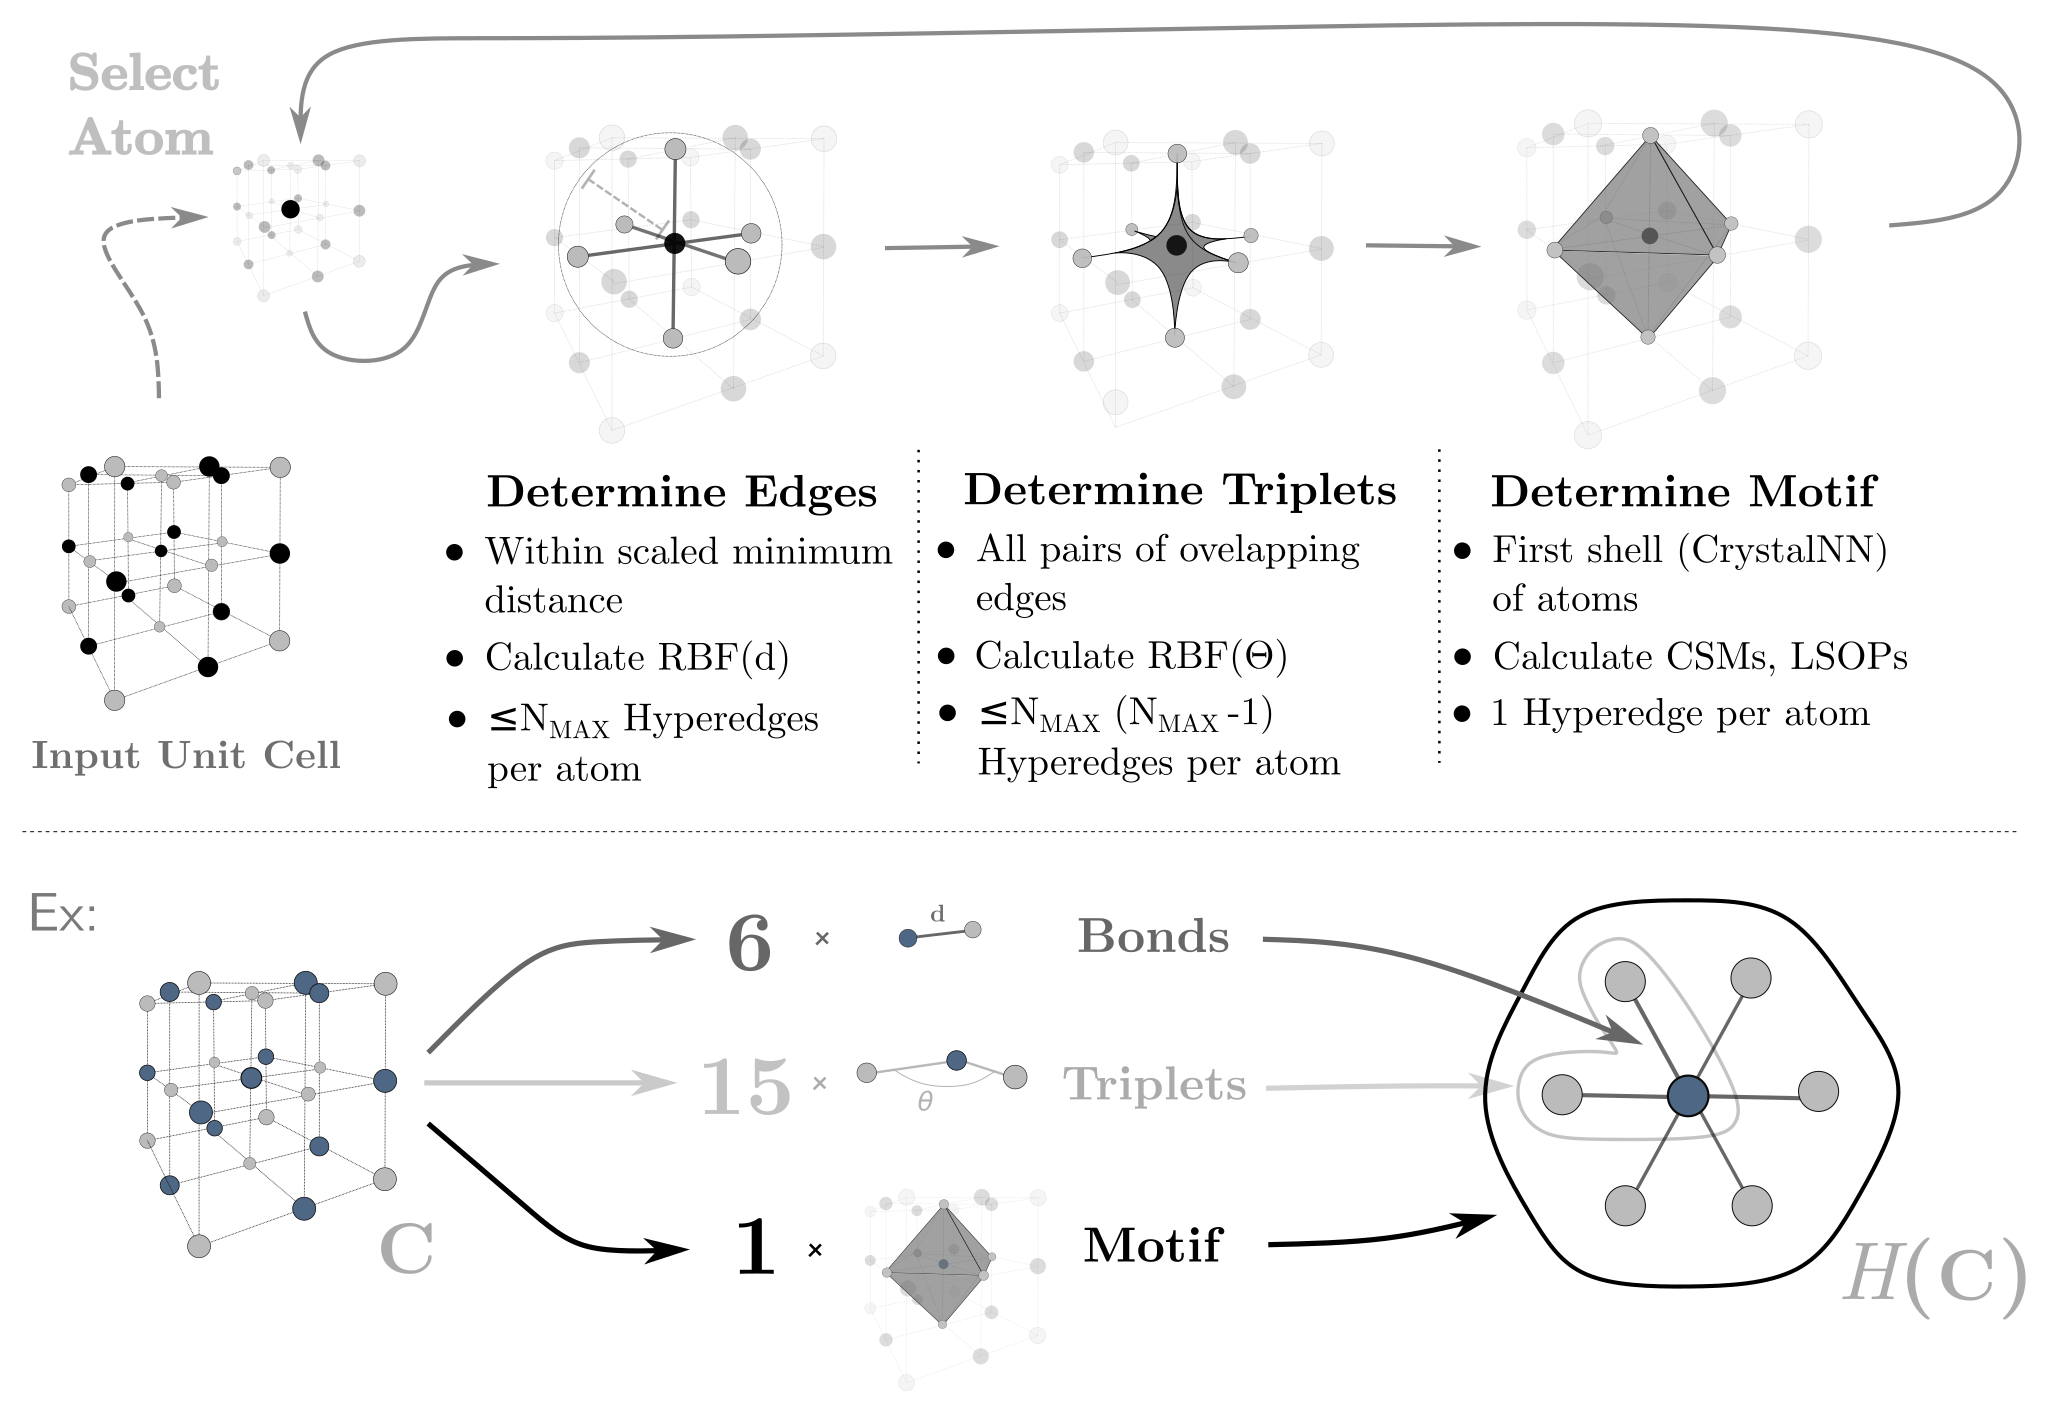
\includegraphics[scale=0.2]{../chgcnn/chgcnn_revised_3/crystal_hgraph_ex+revamp3.pdf}
		\caption{Typical construction loop for a crystal hypergraph. First, pair-wise bonds/edges are determined, then triplets are derived from overlapping pairs of bonds, and finally motifs are determined as first-shells of neighbors by some (generally more restrictive) criteria. Features for each and upper bounds on numbers of hyperedges for each type are also listed. Note that RBF abbreviates radial basis function (such as Gaussian, Bessel, etc.); CSM, continuous symmetry measure; and, LSOP, local structure order parameter.}
		\label{fig:hypergraph-loop}
	\end{figure*}
	
	Each of the aforementioned structures also has a natural set of distinct, coordinate-system invariant features that may be associated with them. At the triplet level (where two bonds share some common node), there is always a corresponding angle. While at the motif level, order parameters \cite{orderparam1, orderparam2} or continuous symmetry measures \cite{csm_polyhedra, chemenv} may be used to describe 3-dimensional coordination environments quantitatively. 
	These different order structures may all be represented in a single crystal hypergraph, and is accounted for by treating the data as a heterogeneous graph, with different hyperedge types.
	
	
	Of course, these different structures require different sets of descriptors, and thus inequivalent feature vectors, suggesting these crystal hypergraphs are naturally heterogeneous in their hyperedges. That is, not all hyperedges in crystal hypergraphs are of the same type. This simply means we need different convolutional filters for each type of hyperedge.
	
	\subsubsection{Crystal Hypergraph Convolution}
	To accomodate these extended representations, we must also consider a new convolutional structure, analogous to \textit{Gilmore, et al} \cite{MPNN} but applying to hypergraph structures. That is, we now have:
	\begin{align*}
		m_v^{t+1}&=\sum_{h_j\in \mathcal{N}(v)} M_t(n_v^{t},h_j^{t},\lbrace n_w^t \vert n_w \in h_j \rbrace),\\
		n_v^{t+1}&=U_t(n_v^t,m_v^{t+1}),\\
		\hat{y}&=R(\lbrace n_v^T\rbrace),
	\end{align*}
	so that each node is still updated according to some layer-wise update function $U_t$, aggregating messages $m^{t+1}$ formed from origin node features, hyperedge features $h_j$, and hyperedge neighborhood features $n_w \in h_j$. This update occurs node-wise and then after $T$ layers, some readout function $R$ is used to output the corresponding predicted value $\hat{y}$, which utilizes the set of learned node features.
	
	
	The biggest difference here is that we now need a message forming function $M_t$ that accounts for a set of node features $\lbrace n_w^t \vert n_w \in h_j \rbrace$ which may vary in size between different hyperedges (even of the same type). This stands in opposition to the case of regular edges, where we are assured a fixed size of two nodes per edge. 
	
	\begin{figure*}[!h]
		\centering
		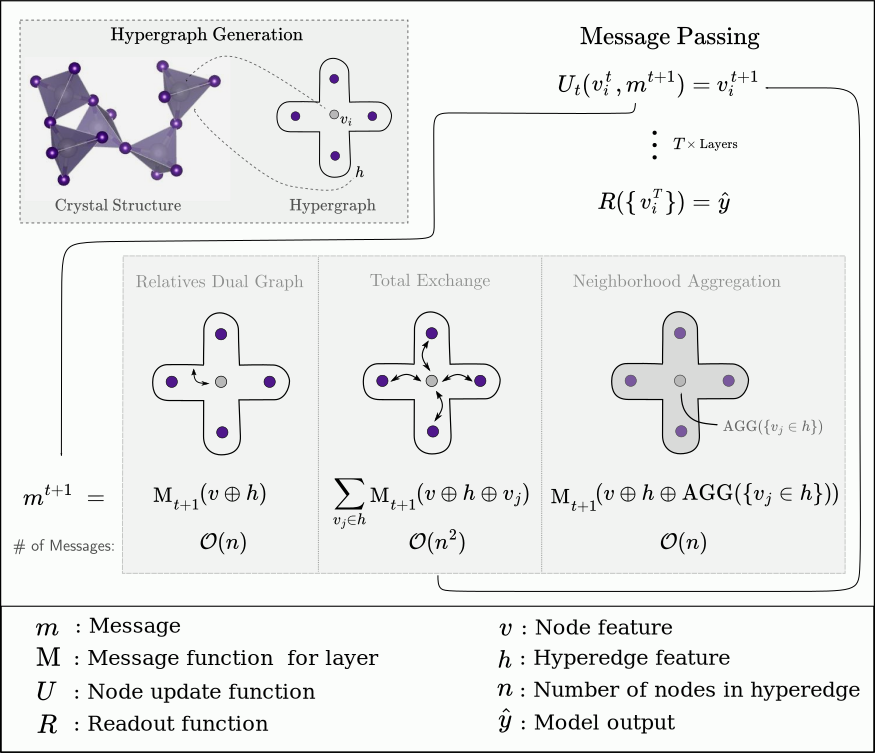
\includegraphics[scale=.45]{../chgcnn/chgcnn_revised_3/HMPNN_loop.pdf}
		\caption{Overview of three possible message functions $M$ for nodes that generalize the message function in \cite{MPNN} to hyperedges $h$ with more (or less) than two nodes. %Here, $n$ represents the average number of nodes in a hyperedge and the scaling relation is for the total number of messages exchanged for each hyperedge, per layer. 
			$\text{AGG}$ specifies some aggregation function acting on the set of node features in the hyperedge, such as max, min, or average.}
		\label{fig:hmpnn}
	\end{figure*}
	
	One approach would be to fix the dimensionality of each type of hyperedge, or have a different convolutional operator for each different size hyperedge (as is effectively the approach taken with line graph networks \cite{linegraph_general}). Here, however, we wish to maintain generality in edge size so we need not fix hyperedge sizes for hyperedge type, since structures of different sizes may be described by similar metrics. For example, we may wish that motifs resembling polyhedra with different numbers of vertices are described by common sets of features. We considered three strategies that allow us to apply our convolutional operator to hyperedges of arbitrary size, with these approaches detailed schematically in   \cref{fig:hmpnn}.

	
	\subsection{Equivariant Tensor Predictions}
	Spherical harmonics, the basis vectors of $O(3)$-invariant subspaces, naturally correspond to sets of basis tensors as well \cite{harmonictensors}. This correspondence allows for the direct prediction of tensorial properties from the output of $O(3)$ networks in a way that respects transformations on the input coordinate system, acting essentially as similar transformations on the output tensors. In this way, $SO(3)$ equivariant networks are naturally well suited for the prediction of tensorial properties. Arbirtrary tensors may generally be decomposed into a set of $SO(3)$ invariant subspaces, which can each be associated with a set of spherical harmonic tensors themselves. Since the outputs of $SO(3)$ networks naturally transform like spherical harmonic tensor coefficients indexed by $\ell$ and $m$, we may then essentially read them off as such and convert these into Cartesian tensor components. In this work \cite{heilman_tensor}, we predicted three common material properties described by tensors, namely: the dielectric tensor for anisotropic materials; the piezoelectric tensor, relating strain to internal electric fields; and the elasticity tensor, relating strain to stress.
	
	The key to such applications is the decomposition of tensor spaces into $\ell$ and $m$ indexed subspaces (that is, into irreducible $SO(3)$ tensor subspaces). 
	Since $SO(3) =   \big( SL(3)\bigcap O(3) \big) \subset GL(3)$, to construct invariants of $SO$, we generally form invariant subspaces under $GL$ by way of Young symmetrizers first, and then construct invariants under $O$ and/or $SL$ of these $GL$ invariant subspaces. This often results in several different harmonic subspaces of the same order $\ell$ in the harmonic decomposition of a tensor.
	Also, note that the $GL$ decompositions for tensors of order greater than two are not, in general, unique and thus $SO(3)$ decompositions of tensors are also often not unique.
	While not the focus of the present work, it should be noted that these three methods correspond to the decomposition of a tensor with respect to the general linear group (by way of Young symmetrizers \cite{young_diagram}), the orthogonal group (contractions with $g_{ij}$), and the special linear group (contractions with $\epsilon_{ijk}$), respectively \cite{itin-elastic, itin-rank3}. These techniques allow one to predict arbitrary tensors of a set rank. However, since these sets form complete basis for arbitrary tensors, symmetries of the material are often not captured through convolution, and thus the model predicts non-zero tensor components that are known to be zero a priori from symmetry constraints.
	
	
	\begin{figure*}[t]
		\begin{center}
			
			\includegraphics[scale=.28]{../spherical-elastic/bigfig.pdf}
		\end{center}
		\caption{Overview of $SO(3)$ decomposition of order two tensors, piezoelectric (order 3) tensors, and elasticity (order 4) tensors. Grey corresponds to scalar subspaces of the related tensor space, blue to order 1 subspaces, purple to order 2, and yellow to order 4. A schematic for the general model architecture used in this work is also provided, where the output coefficients correspond directly to harmonic tensor components resulting from these decompositions.}\label{rank2example}
	\end{figure*}
	

	
	
	
	
	\section{Proposed Project}
	$O(3)$-Equivariant networks have proven effective in applications within the physical sciences, suggesting that physical symmetries are a useful inductive bias in the design of machine learning techniques. While $O(3)$ networks, in principle, can fully incorporate all possible symmetries of a system, in some applications specific symmetry subgroups may be more relevant. One case of this is applications of machine learning to condensed matter systems, where atoms are arranged in periodic structures where each atomic position has some point symmetry group.
	
	In $O(3)$ Equivariant networks, initial edge features $\vec{e}_{ij}^{L=0}$ are often spherical harmonic functions $Y_{m}^{\ell}(\vec{r}_{ab})$ evaluated for interatomic radii $\vec{r}_{ab}$ of atom pairs $(a,b)$. Point group features may be similarly derived from interatomic radii by way of projection operators $\hat{P}_{ij}^{\mu}$  which project arbitrary vector spaces onto subspaces $V_{\mu}$ transforming as irreducible representations $\mu$ of point group $G$, and defined as \cite{projection_op}:
	$$
	\hat{P}_{\alpha}^{kk} = \frac{d_{\alpha}}{N}\sum_g \big[\Gamma_{kk}^{\alpha}(g) \big]^* O(g)
	$$
	where $d_{\alpha}$ is the dimension of irrep $\Gamma^{\alpha}$, $N$ is the order of the group, and $O(g)$ is the operator representation acting on the feature space of relevance.
	While $O(3)$ networks rely on Clebsch-Gordan expansions of tensor products of neighboring sites and filters, point group networks instead require generalized CG coefficients or `coupling coefficients' $U^{\gamma n}_{\alpha i \beta j}$ for the direct sum decompositions of point group-irreducible features:
	$$
	\psi_{n}^{\gamma} = \bigoplus_{\alpha i,\beta j} U^{\gamma n}_{\alpha i \beta j} \big( u^{\alpha}_i\otimes v_{j}^{\beta}\big)
	$$
	With these coefficients, a similar convolutional structure may be adopted, as in $O(3)$ networks, though now instead of harmonic indices $\ell,m$ for features, we have point group irreducible representation indices $\gamma, n$:
	$$
	\big(v^{L+1}_{nc}\big) ^{\gamma}_{n}=\big(v^{L}_{nc}\big)^{\gamma}_n+\sum_{b\in \mathcal{N}(n)}\sum_{\alpha i, \beta j}U_{\alpha i \beta j}^{\gamma n}\big(F^{L}_c(r_{nb})\big)^{\beta }_{j}\big(v_{bc}^L \big)^{\alpha}_{i}
	$$
	The implementation of these models requires the availability of the analagous Clebsch-Gordan coefficients, $U^{\gamma n}_{\alpha i \beta j}$, which we refer to more generally as \textit{coupling coefficients}, for all point groups of interest. These may be defined, from particular forms of representations $\Gamma^{\alpha},\Gamma^{\beta},\Gamma^{\gamma}$ for all point groups of interest from Dirl's formula \cite{dirl1979}:
	$$
	(U^{\gamma n}_{\alpha i \beta j})^m = \sqrt{\frac{d_{\gamma}}{N_{G}}}\Big(\sum_{g\in G}\Gamma^{\alpha}_{qq}(g)\Gamma^{\beta}_{ss}(g)\Gamma^{\gamma \dagger}_{aa}(g)\Big)^{-\frac{1}{2}}\cdot \sum_{g\in G}\Gamma^{\alpha}_{iq}(g)\Gamma^{\beta}_{js}(g)\Gamma^{\gamma\dagger}_{na}(g)
	$$
	It should be noted here that the definition of these coefficients thus requires explicit (fixed) forms for each irrep of each point group of interest.
	
	We propose to incorporate the above techniques into a novel framework for point-group-equivariant graph networks, suited for applications where systems display particular symmetries reduced from the full rotation symmetry of $O(3)$. One particularly relevant application is the prediction of condensed matter Hamiltonian elements. In solid-state systems based upon an underlying periodic lattice, each atomic position displays a certain point group symmetry. Thus the Hamiltonian of the system must share a simultaneous set of eigenvalues with the symmetry operations since in this case they necessarily commute. Essentially then, the Hamiltonians solutions must be indexed by the same set as the irreducible subspaces $V_{\mu}$, each of dimension $d_{\mu}$. The basis set of one-particle wavefunctions then must have a separable form:
	$$
	\psi^{\mu}_{nm}(\vec{r})=R_{\mu n m}(r)\Omega^{\mu}_n(\theta,\phi)
	$$
	where $1\leq n\leq d_{\mu}$. The radial function $R_{\mu n m}(r)$ then depends on the specific form of the Hamiltionian and may have a very complicated structure. The prediction of this functional dependence is thus well suited for the machine learning applications discussed here. Such models provide a method by which we may predict Hamiltionian elements naturally associated with these point-group indexes, allowing for complete descriptions of interactions between neighboring sites irreducible subspaces without truncations of rotational order (such as $\ell_{max}$ in $O(3)$ networks). 
	
	Furthermore, these models allow for the prediction of properties that respect the known symmetries of physical systems, by reading out features that transform as the trivial representation, allowing for more intuitive predictions of scalar (totally invariant) quantities from input directional quantities, as well as tensorial properties with desired physical symmetries.
	
	A natural starting point for such applications is to material systems with high symmetry, the largest crystalline point group being $O_h$ with 48 operations (including rotations, inversion, and mirror planes). The Materials Project database \cite{matproj} contains approximately 15,000 crystalline materials with such $O_h$ symmetry, constituting a suitably large training set for some basic machine learning tasks. 
	
	However, while scalar targets, such as band gap, formation energy, and metalicity are generally available from the Materials Project along with the corresponding crystal structures, one large difficulty with this project will be the availability of data for Hamiltonian matrix elements in a properly symmetrized basis (which is also required to be localized in real space). This may possibly be approached by generating such data using a symmetry-adapted Wannier basis with DFT \cite{symmetry_wannier}.
	
	%Equivariance under the total rotation group (or the total group of translations and rotations) is now well-implemented and widely used. However, for many atomic systems, $O(3)$ equivariance is, in a certain sense, too large a set of symmetries to consider. For example, in a cubic crystalline system, one may wish to predict the ground-state electronic orbitals, and a priori, enforce there should be no $\ell=3,\ m=3$ states due to the symmetry of the system. While one may simply mask the output of the model to enforce such symmetries, such considerations are not always so straight-forward. A relevant further example is the prediction of material properties represented by tensorial quantities. In systems with certain crystalline symmetries several components necessarily vanish, and models have no way to directly enforce these symmetries from their design outside of masking and group averaging.
	
	%To cure these ails of $O(3)$-equivariant networks, we propose \textit{point group equivariant networks}, which instead preserve equivariance under the group of symmetry operations of atomic sites. Such models, by their construction, allow for the readout of symmetry group invariant quantities by simply reading off the outputs associated with trivial representations (analagous to the $\ell=0$ channel of rotationally-equivariant networks).
	
	%\section{Methods \& Timeline}

	\printbibliography

\end{document}          
